\documentclass{beamer}

\usecolortheme[light]{solarized}

\beamertemplatenavigationsymbolsempty

\usepackage{hyperref}

\usepackage{booktabs}
\usepackage{graphicx}
\usepackage{minted}
\usepackage{moresize}
\usepackage{standalone}
\usepackage{tcolorbox}
\usepackage{tikz}
\usepackage[normalem]{ulem}
\usepackage{xpatch}
\usepackage{amsmath}

\xpatchcmd{\sout}
  {\bgroup}
    {\bgroup\def\ULthickness{2pt}}
      {}{}

\usetikzlibrary{calc, patterns}

\definecolor{twitter}{RGB}{64, 153, 255}
\definecolor{github}{RGB}{211, 211, 211}


\begin{document}

    \begin{frame}
        \begin{center}
            \Large
            The Mathematics of Evolution
        \end{center}

    \end{frame}

    \begin{frame}
        \begin{center}
            \scalebox{.6}{\documentclass{standalone}
\usepackage{tikz}
\usetikzlibrary{calc, shapes, patterns}

\begin{document}
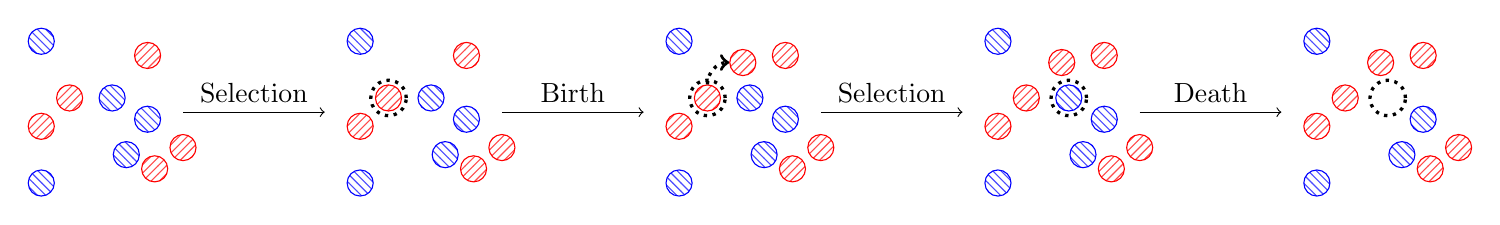
\begin{tikzpicture}[scale=.9]
	\node (A1) at (-1, -1) [circle, pattern=north west lines, pattern
        color=blue!70, draw=blue] {};
	\node (A2) at (-1, 1) [circle, pattern=north west lines, pattern
        color=blue!70, draw=blue] {};
	\node (A3) at (0, .2) [circle, pattern=north west lines, pattern
        color=blue!70, draw=blue] {};
	\node (A4) at (.2, -.6) [circle, pattern=north west lines, pattern
        color=blue!70, draw=blue] {};
	\node (A5) at (.5, -0.1) [circle, pattern=north west lines, pattern
        color=blue!70, draw=blue] {};
	\node (B1) at (-1, -.2) [circle, pattern=north east lines, pattern
        color=red!70, draw=red] {};
	\node (B2) at (1, -.5) [circle, pattern=north east lines, pattern
        color=red!70, draw=red] {};
	\node (B3) at (.5, .8) [circle, pattern=north east lines, pattern
        color=red!70, draw=red] {};
	\node (B4) at (-.6, .2) [circle, pattern=north east lines, pattern
        color=red!70, draw=red] {};
	\node (B5) at (.6, -.8) [circle, pattern=north east lines, pattern
        color=red!70, draw=red] {};

	\draw [->] (1, 0) -- (3, 0) node [above, pos=0.5] {Selection};

	\node (A1) at ($(A1) + (4.5, 0)$) [circle, pattern=north west lines,
        pattern color=blue!70, draw=blue] {};
	\node (A2) at ($(A2) + (4.5, 0)$) [circle, pattern=north west lines,
        pattern color=blue!70, draw=blue] {};
	\node (A3) at ($(A3) + (4.5, 0)$) [circle, pattern=north west lines,
        pattern color=blue!70, draw=blue] {};
	\node (A4) at ($(A4) + (4.5, 0)$) [circle, pattern=north west lines,
        pattern color=blue!70, draw=blue] {};
    \node (A5) at ($(A5) + (4.5, 0)$) [circle, pattern=north west lines,
        pattern color=blue!70, draw=blue] {};
	\node (B1) at ($(B1) + (4.5, 0)$) [circle, pattern=north east lines,
        pattern color=red!70, draw=red] {};
	\node (B2) at ($(B2) + (4.5, 0)$) [circle, pattern=north east lines,
        pattern color=red!70, draw=red] {};
	\node (B3) at ($(B3) + (4.5, 0)$) [circle, pattern=north east lines,
        pattern color=red!70, draw=red] {};
	\node (B4) at ($(B4) + (4.5, 0)$) [circle, pattern=north east lines,
        pattern color=red!70, draw=red] {};
	\node (B5) at ($(B5) + (4.5, 0)$) [circle, pattern=north east lines,
        pattern color=red!70, draw=red] {};

	\draw [dotted, very thick] (B4) circle (.25cm);

	\draw [->] (5.5, 0) -- (7.5, 0) node [above, pos=0.5] {Birth};

	\node (A1) at ($(A1) + (4.5, 0)$) [circle, pattern=north west lines,
        pattern color=blue!70, draw=blue] {};
	\node (A2) at ($(A2) + (4.5, 0)$) [circle, pattern=north west lines,
        pattern color=blue!70, draw=blue] {};
	\node (A3) at ($(A3) + (4.5, 0)$) [circle, pattern=north west lines,
        pattern color=blue!70, draw=blue] {};
	\node (A4) at ($(A4) + (4.5, 0)$) [circle, pattern=north west lines,
        pattern color=blue!70, draw=blue] {};
    \node (A5) at ($(A5) + (4.5, 0)$) [circle, pattern=north west lines,
        pattern color=blue!70, draw=blue] {};
	\node (B1) at ($(B1) + (4.5, 0)$) [circle, pattern=north east lines,
        pattern color=red!70, draw=red] {};
	\node (B2) at ($(B2) + (4.5, 0)$) [circle, pattern=north east lines,
        pattern color=red!70, draw=red] {};
	\node (B3) at ($(B3) + (4.5, 0)$) [circle, pattern=north east lines,
        pattern color=red!70, draw=red] {};
	\node (B4) at ($(B4) + (4.5, 0)$) [circle, pattern=north east lines,
        pattern color=red!70, draw=red] {};
	\node (B5) at ($(B5) + (4.5, 0)$) [circle, pattern=north east lines,
        pattern color=red!70, draw=red] {};

	\draw [dotted, very thick] (B4) circle (.25cm);
	\node (B6) at ($(B4) + (0.5, 0.5)$) [circle, pattern=north east lines,
        pattern color=red!70, draw=red] {};
	\draw [->, dotted, very thick] (B4) [out=90, in=180] to (B6);

	\draw [->] (10, 0) -- (12, 0) node [above, pos=0.5] {Selection};

	\node (A1) at ($(A1) + (4.5, 0)$) [circle, pattern=north west lines,
        pattern color=blue!70, draw=blue] {};
	\node (A2) at ($(A2) + (4.5, 0)$) [circle, pattern=north west lines,
        pattern color=blue!70, draw=blue] {};
	\node (A3) at ($(A3) + (4.5, 0)$) [circle, pattern=north west lines,
        pattern color=blue!70, draw=blue] {};
	\node (A4) at ($(A4) + (4.5, 0)$) [circle, pattern=north west lines,
        pattern color=blue!70, draw=blue] {};
    \node (A5) at ($(A5) + (4.5, 0)$) [circle, pattern=north west lines,
        pattern color=blue!70, draw=blue] {};
	\node (B1) at ($(B1) + (4.5, 0)$) [circle, pattern=north east lines,
        pattern color=red!70, draw=red] {};
	\node (B2) at ($(B2) + (4.5, 0)$) [circle, pattern=north east lines,
        pattern color=red!70, draw=red] {};
	\node (B3) at ($(B3) + (4.5, 0)$) [circle, pattern=north east lines,
        pattern color=red!70, draw=red] {};
	\node (B4) at ($(B4) + (4.5, 0)$) [circle, pattern=north east lines,
        pattern color=red!70, draw=red] {};
	\node (B5) at ($(B5) + (4.5, 0)$) [circle, pattern=north east lines,
        pattern color=red!70, draw=red] {};
	\node (B6) at ($(B6) + (4.5, 0)$) [circle, pattern=north east lines,
        pattern color=red!70, draw=red] {};

	\draw [dotted, very thick] (A3) circle (.25cm);

	\draw [->] (14.5, 0) -- (16.5, 0) node [above, pos=0.5] {Death};

	\node (A1) at ($(A1) + (4.5, 0)$) [circle, pattern=north west lines,
        pattern color=blue!70, draw=blue] {};
	\node (A2) at ($(A2) + (4.5, 0)$) [circle, pattern=north west lines,
        pattern color=blue!70, draw=blue] {};
	\node (A3) at ($(A3) + (4.5, 0)$) {};
	\node (A4) at ($(A4) + (4.5, 0)$) [circle, pattern=north west lines,
        pattern color=blue!70, draw=blue] {};
    \node (A5) at ($(A5) + (4.5, 0)$) [circle, pattern=north west lines,
        pattern color=blue!70, draw=blue] {};
	\node (B1) at ($(B1) + (4.5, 0)$) [circle, pattern=north east lines,
        pattern color=red!70, draw=red] {};
	\node (B2) at ($(B2) + (4.5, 0)$) [circle, pattern=north east lines,
        pattern color=red!70, draw=red] {};
	\node (B3) at ($(B3) + (4.5, 0)$) [circle, pattern=north east lines,
        pattern color=red!70, draw=red] {};
	\node (B4) at ($(B4) + (4.5, 0)$) [circle, pattern=north east lines,
        pattern color=red!70, draw=red] {};
	\node (B5) at ($(B5) + (4.5, 0)$) [circle, pattern=north east lines,
        pattern color=red!70, draw=red] {};
	\node (B6) at ($(B6) + (4.5, 0)$) [circle, pattern=north east lines,
        pattern color=red!70, draw=red] {};

	\draw [dotted, very thick] (A3) circle (.25cm);
\end{tikzpicture}
\end{document}
}
            % TODO Possibly re draw.
        \end{center}

		\pause

		  \begin{align*}
			  p_{i, i-1}&=\frac{i(N - i)}{N^2}\\
			  p_{i, i+1}&=\frac{i(N - i)}{N^2}\\
			  p_{i, i}&=1 - p_{i, i-1} - p_{i, i+1}
		  \end{align*}

    \end{frame}

\begin{frame}
    \Huge
    \[
        \begin{pmatrix}
            0 & 3\\
            1 & 2
        \end{pmatrix}
    \]
\end{frame}

\begin{frame}
    \Huge
    \begin{center}
        Group simulation
    \end{center}
\end{frame}

\begin{frame}
   \begin{align*}
       f_{1i} &= \frac{3(N-i)}{N - 1}=3\frac{N-i}{N-1}\\
       f_{2i} &= \frac{i+2(N - i -1)}{N - 1}=\frac{2N-2-i}{N - 1}\\
   \end{align*}

   \[
   x_1 = \frac{1}{1 + 5/9 + 5/9\times2/3 +5/9\times2/3\times1}=\frac{1}{62/27}=\frac{27}{62}\approx.44
   \]
\end{frame}

\begin{frame}
    \Huge
    \begin{center}
        Computer simulation
    \end{center}
\end{frame}

\end{document}
